\section{Mesures}

\begin{frame}{Dispositif de mesure}
\begin{figure}
\centering
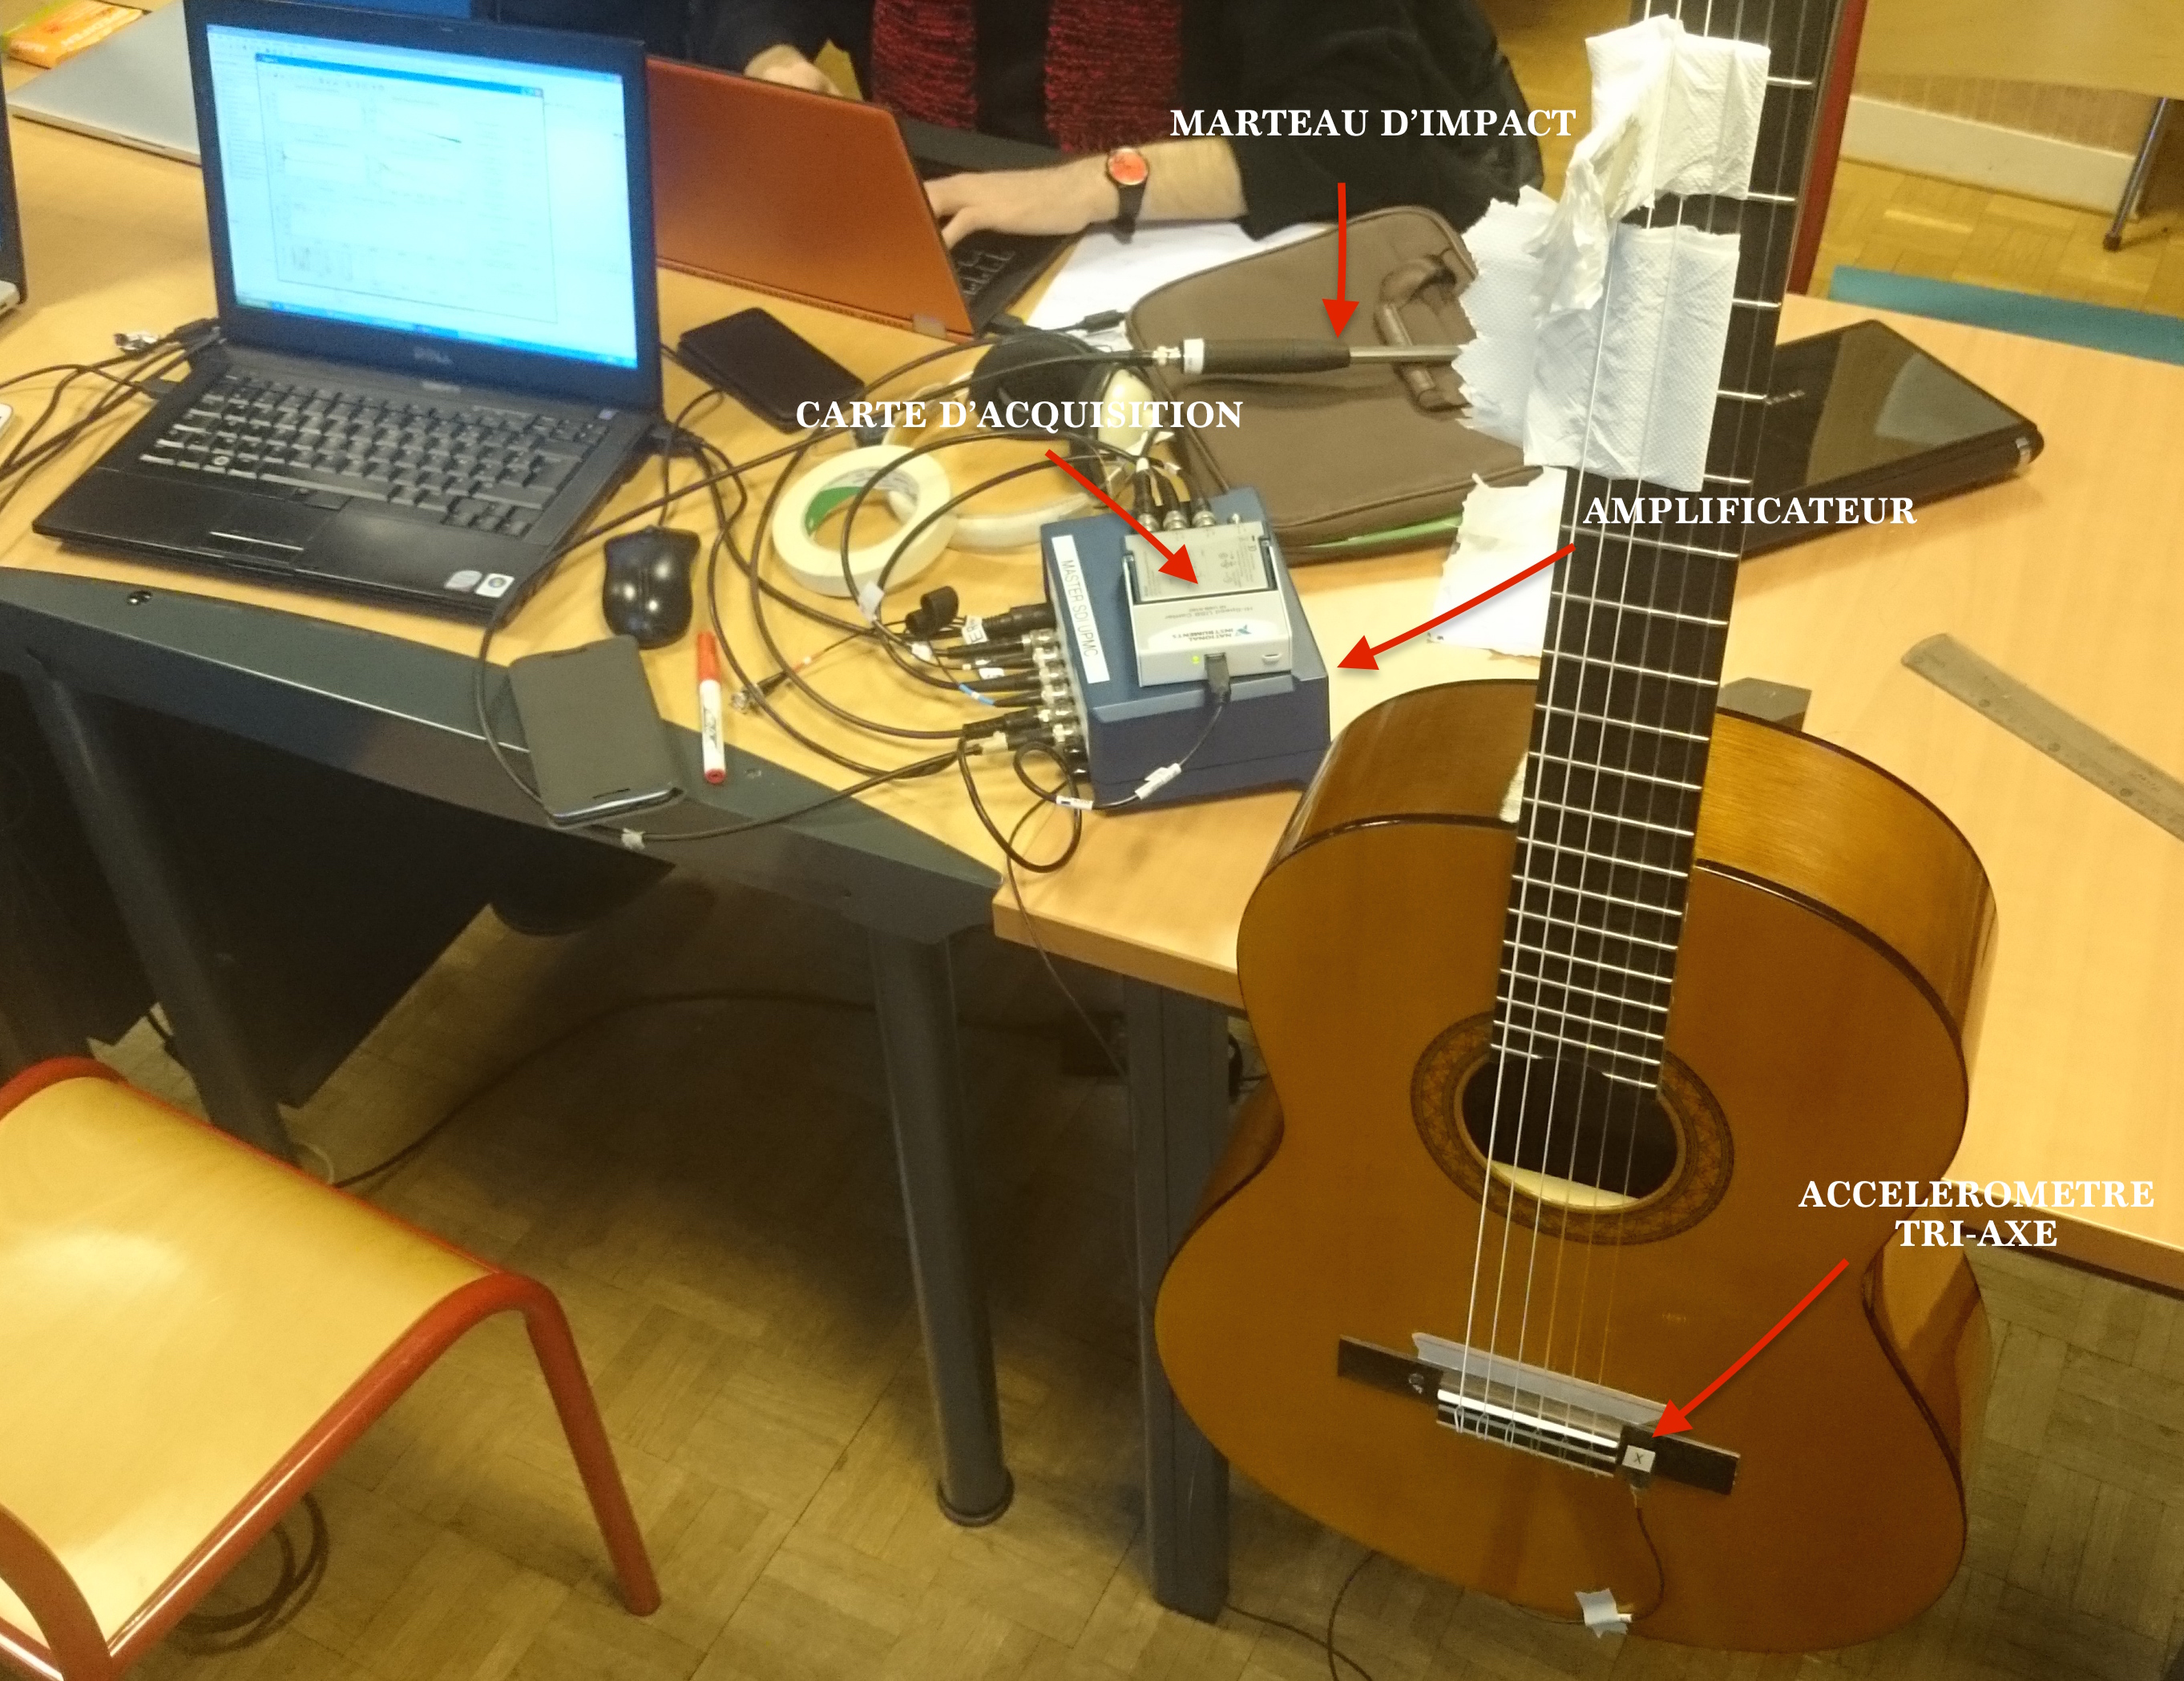
\includegraphics[width = 8cm]{figures/dispo.JPG}
\end{figure}
\end{frame}

 \begin{frame}{Protocole de mesure} 
  \begin{itemize}
  	\item Mesures d'inertance (accélération sur force) de corps et des deux cordes de Mi,
  	\item Types d'excitation : marteau et fil de cuivre.
%     \item Etude de la cohérence mesure au marteau.
    \begin{figure}
		\centering
		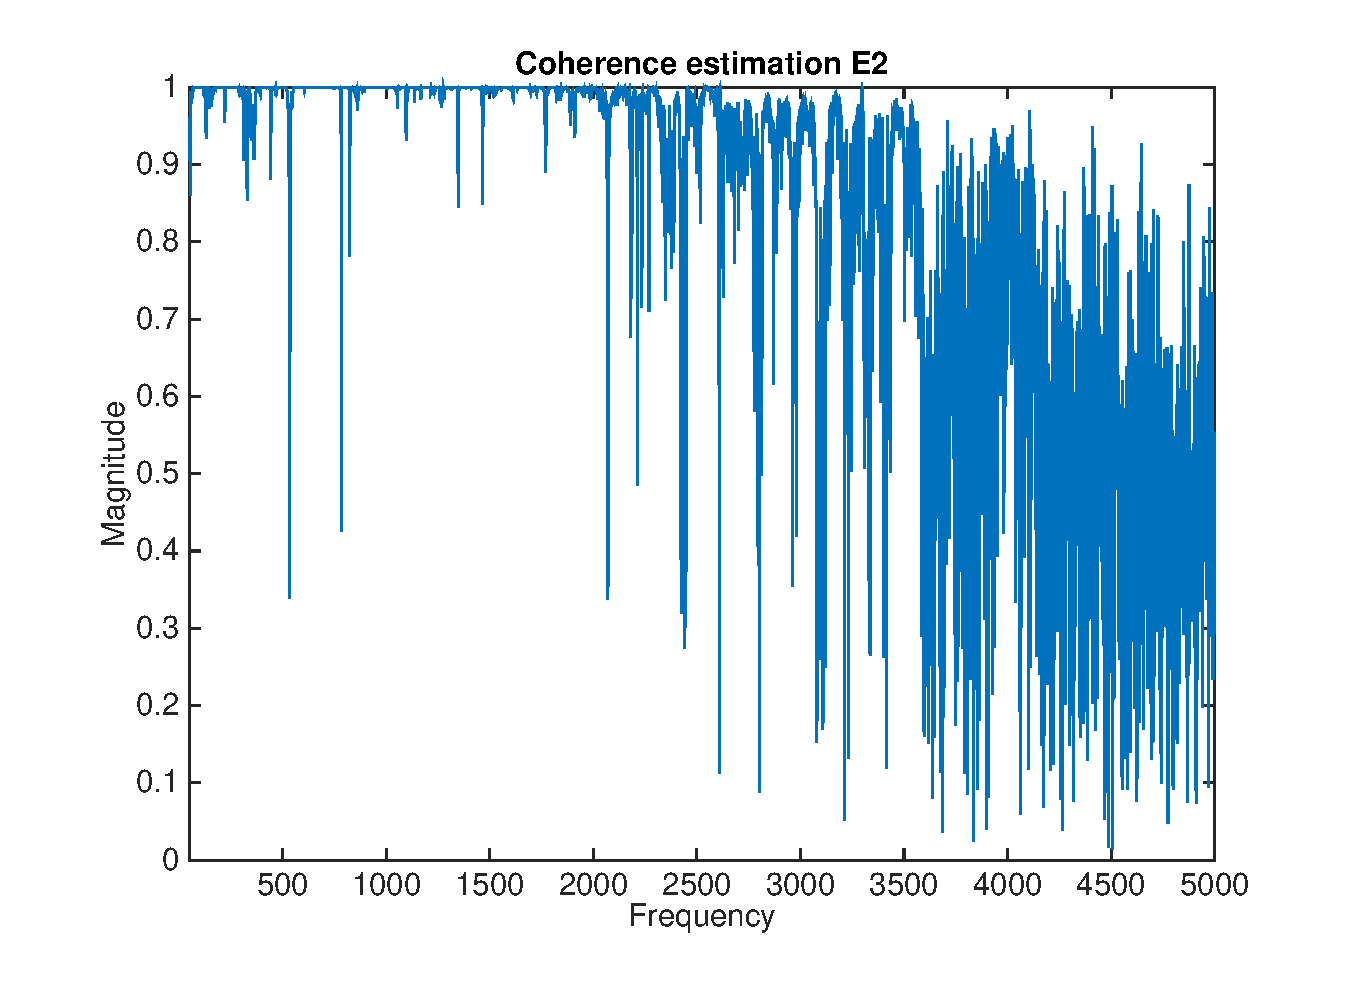
\includegraphics[width = 4.5cm]{figures/coherence_Z_1_E2.eps}
	\caption{Cohérence de la mesure au marteau}
	\end{figure}
  \item Application d'ESPRIT.
  \end{itemize} 
 \end{frame}